\documentclass[a4paper,10pt]{report}
\usepackage[T1]{fontenc}
\usepackage[utf8]{inputenc}
\usepackage{lmodern}
\usepackage[francais]{babel}
\usepackage{amsmath} % math
\usepackage{amssymb} % math
\usepackage{gensymb} % math
\usepackage{graphicx} % images
% \usepackage{qtree}    % dessiner des arbres %% => texlive-humanities
\usepackage{url}
\urlstyle{sf}
\usepackage{multicol} % for multicolonm
\usepackage{subfig} % for subfigure
\usepackage[usenames]{color}
\usepackage[french]{varioref} % \vpageref
\usepackage[top=2.5cm, bottom=2.5cm, left=2.5cm, right=2.5cm]{geometry}
\definecolor{codeBlue}{rgb}{0,0,1}
\definecolor{webred}{rgb}{0.5,0,0}
\definecolor{codeGreen}{rgb}{0,0.5,0}
\definecolor{codeGrey}{rgb}{0.6,0.6,0.6}
\definecolor{webdarkblue}{rgb}{0,0,0.4}
\definecolor{webgreen}{rgb}{0,0.3,0}
\definecolor{webblue}{rgb}{0,0,0.8}
\definecolor{orange}{rgb}{0.7,0.1,0.1}
\usepackage{caption}
\renewcommand{\familydefault}{\sfdefault}
\usepackage{listings}        % Pour l'insersion de fichiers de codes sources.
\lstset{
      language=Java,
      flexiblecolumns=true,
      numbers=left,
      stepnumber=1,
      numberstyle=\ttfamily\tiny,
      keywordstyle=\ttfamily\textcolor{blue},
      stringstyle=\ttfamily\textcolor{red},
      commentstyle=\ttfamily\textcolor{green},
      breaklines=true,
      extendedchars=true,
      basicstyle=\ttfamily\scriptsize,
      showstringspaces=false
    }
%%%%%%%%%%%%%%%%%%%%
\title{Bouboule - Manual}
\author{Matthieu \textsc{Baerts} \and Baptiste \textsc{Remy} \and Nicolas \textsc{Van Wallendael} \and Hélène \textsc{Verhaeghe}}
    \date{\today}
\begin{document}
\maketitle

\section*{Description of the different views}

\begin{figure} [h!]
	\centering
	\subfloat[Main menu]{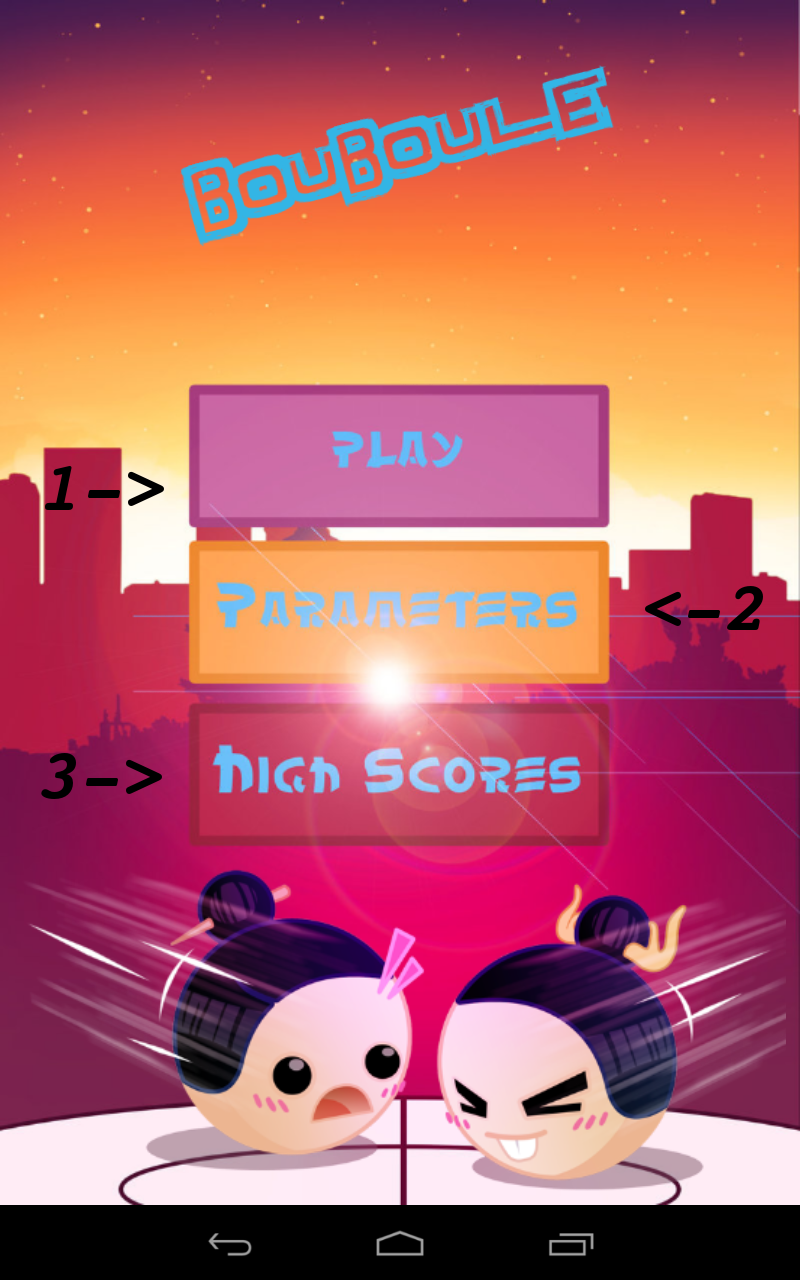
\includegraphics[scale=0.15]{1_Menu.png}}
	\subfloat[World selector]{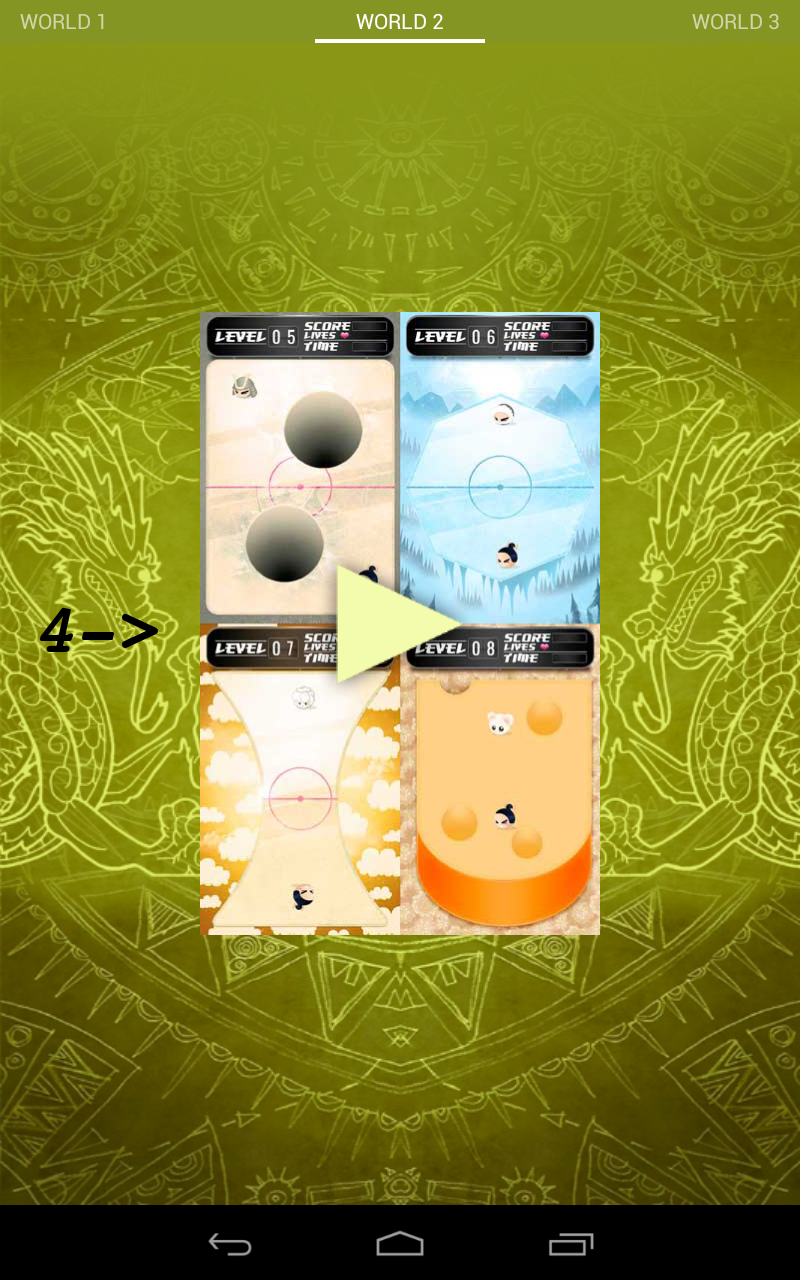
\includegraphics[scale=0.15]{2_WorldSelector.png}}
	\subfloat[Game]{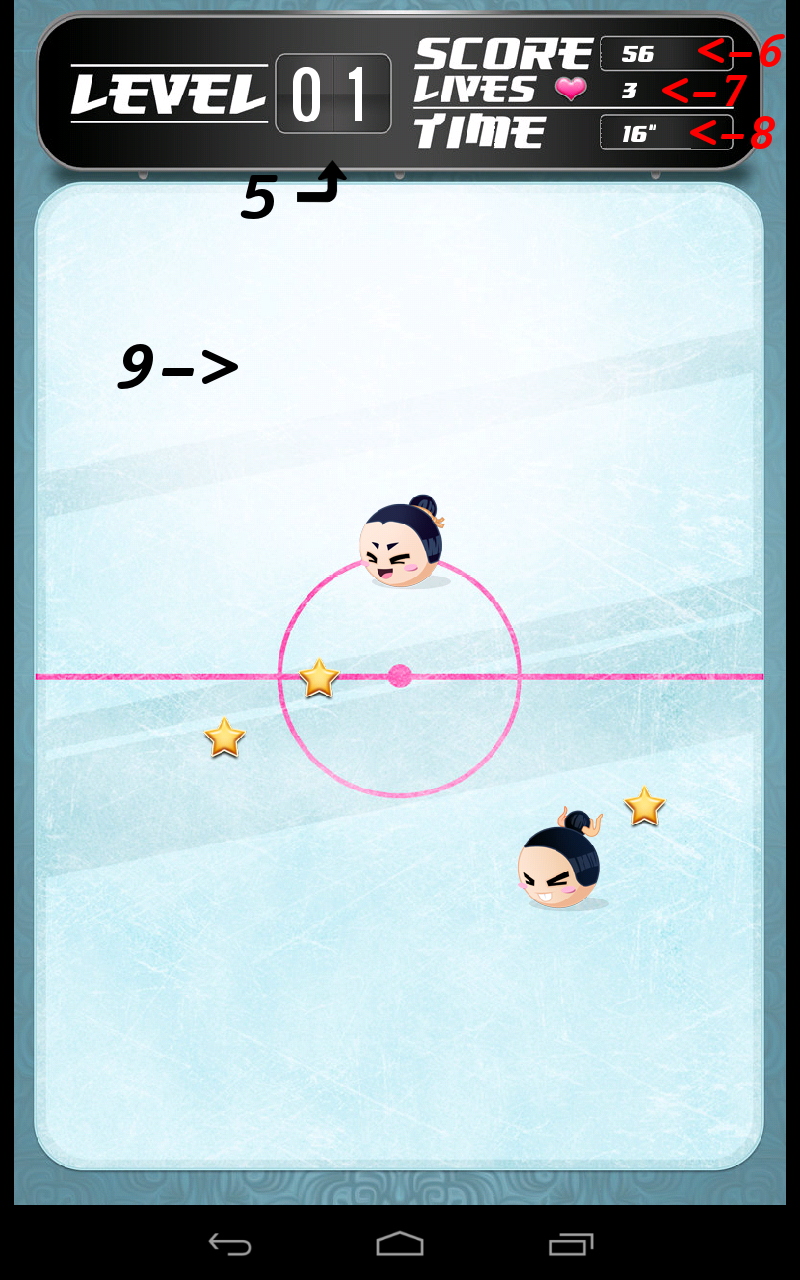
\includegraphics[scale=0.15]{3_Game.png}}\\
	\subfloat[Winning screen]{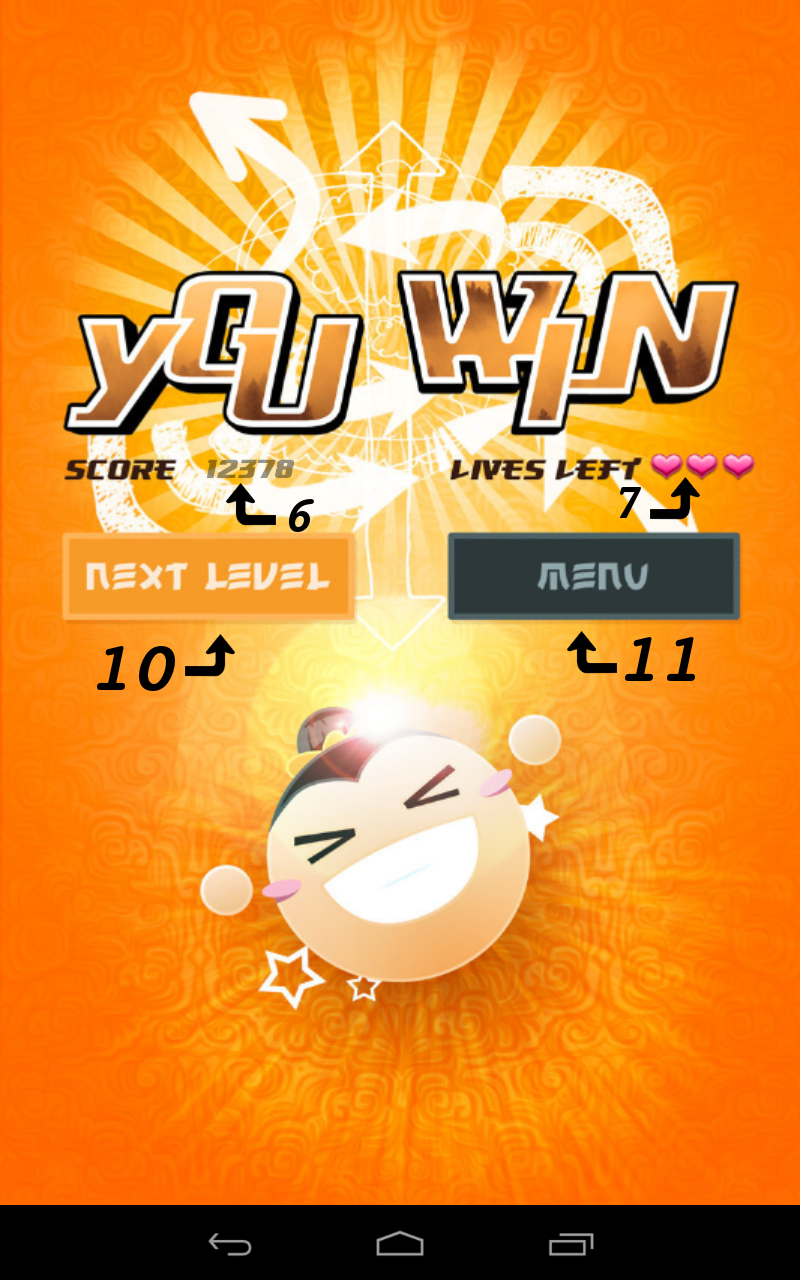
\includegraphics[scale=0.15]{4_Win.png}}
	\subfloat[Losing screen]{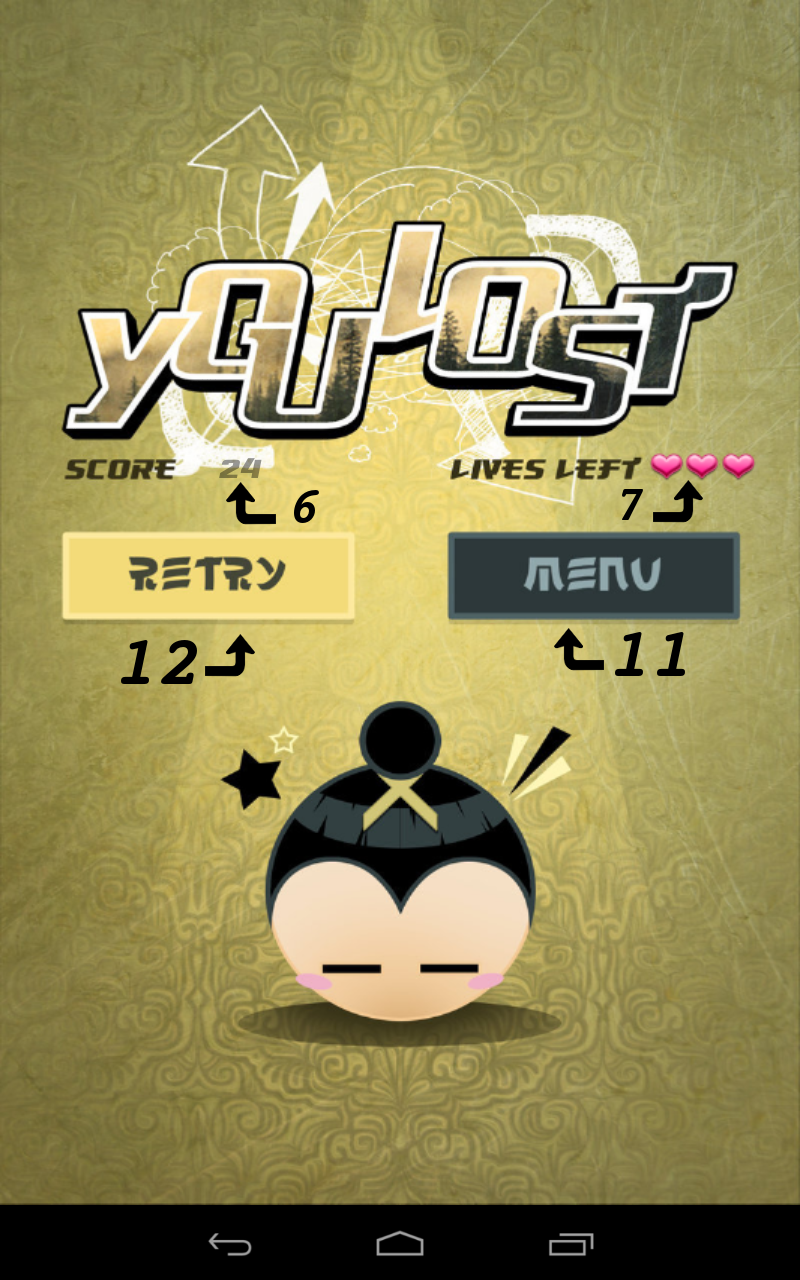
\includegraphics[scale=0.15]{5_Lost.png}}
	\subfloat[Game over screen]{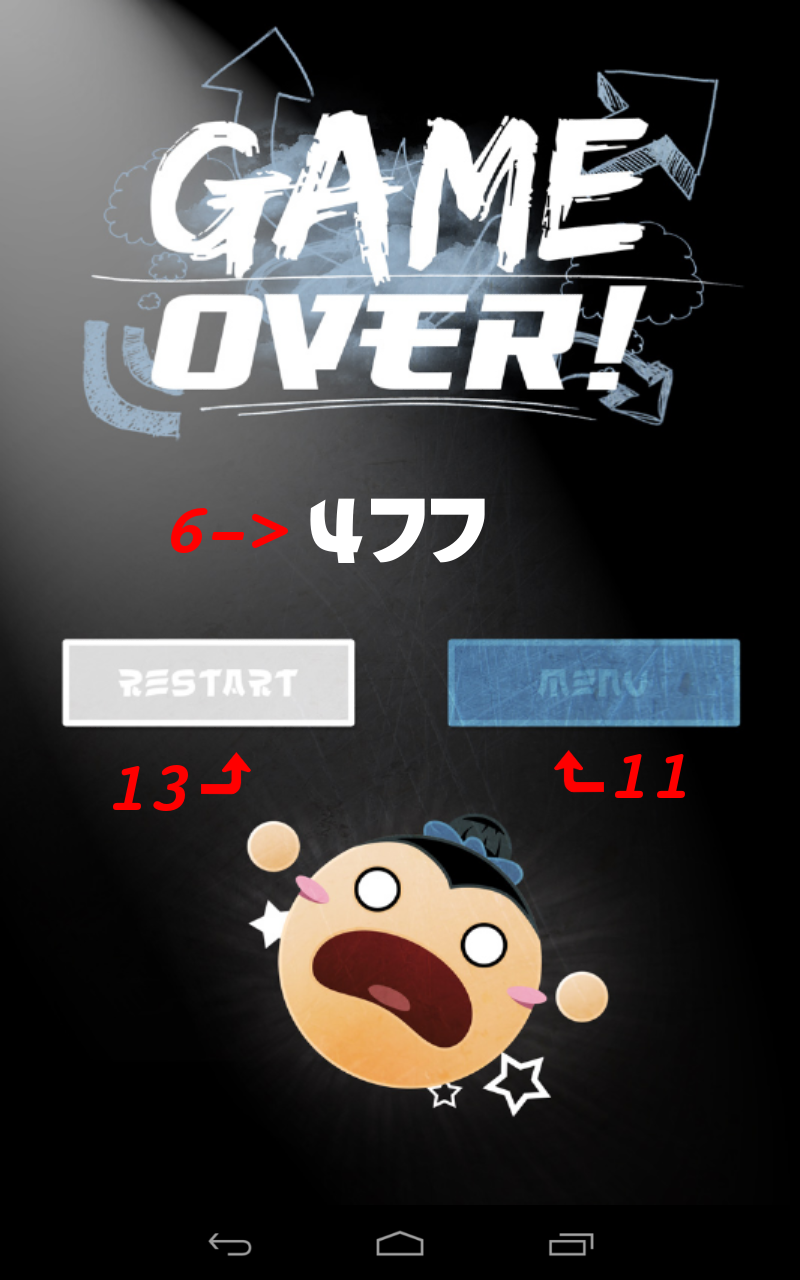
\includegraphics[scale=0.15]{6_GameOver.png}}\\
	\subfloat[Settings menu]{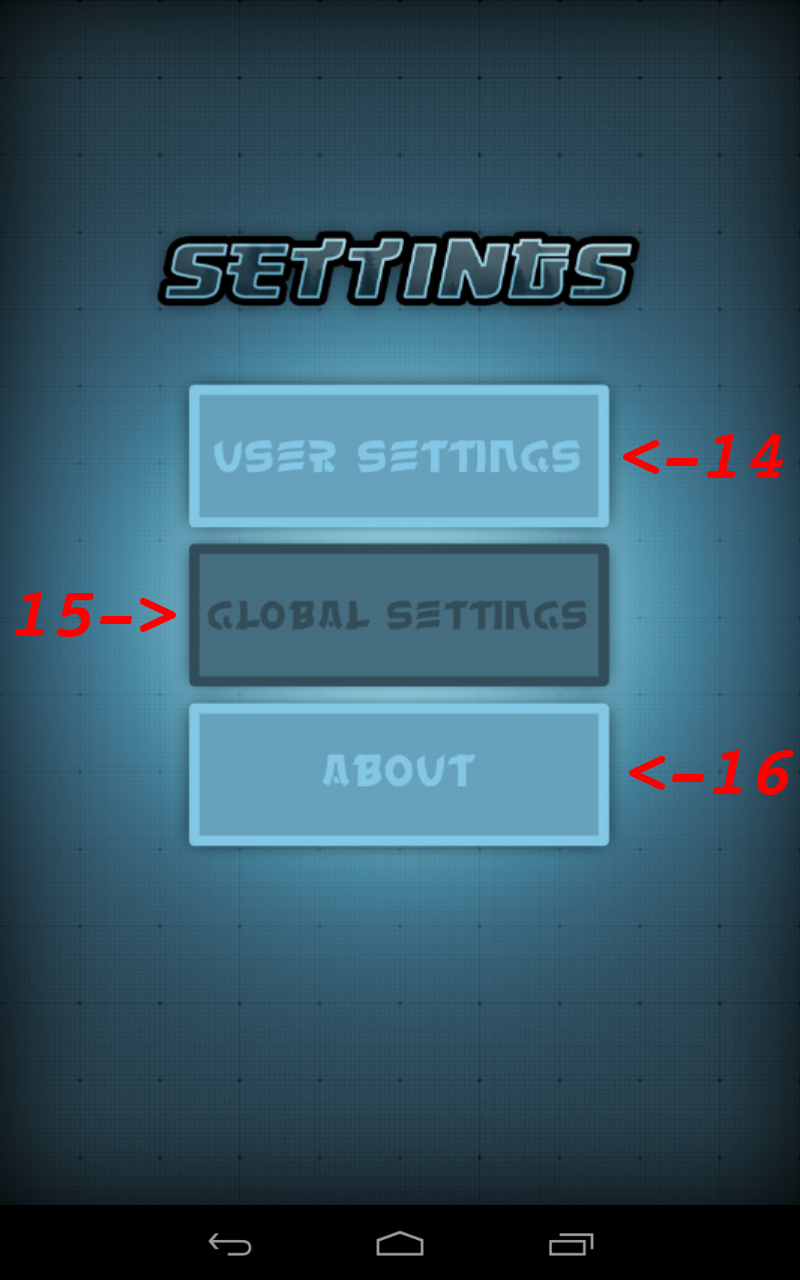
\includegraphics[scale=0.15]{7_Settings.png}}
	\subfloat[User settings menu]{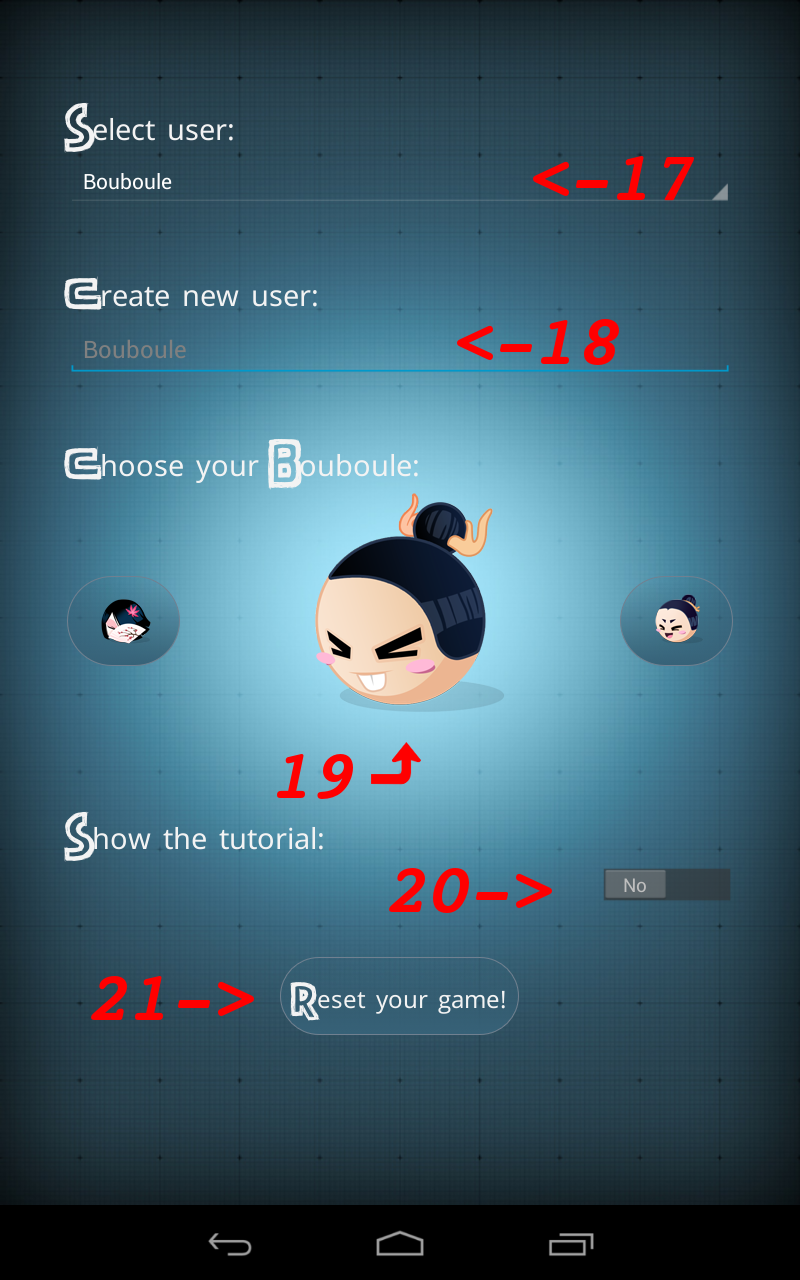
\includegraphics[scale=0.15]{8_UserSettings.png}}
	\subfloat[Global settings menu]{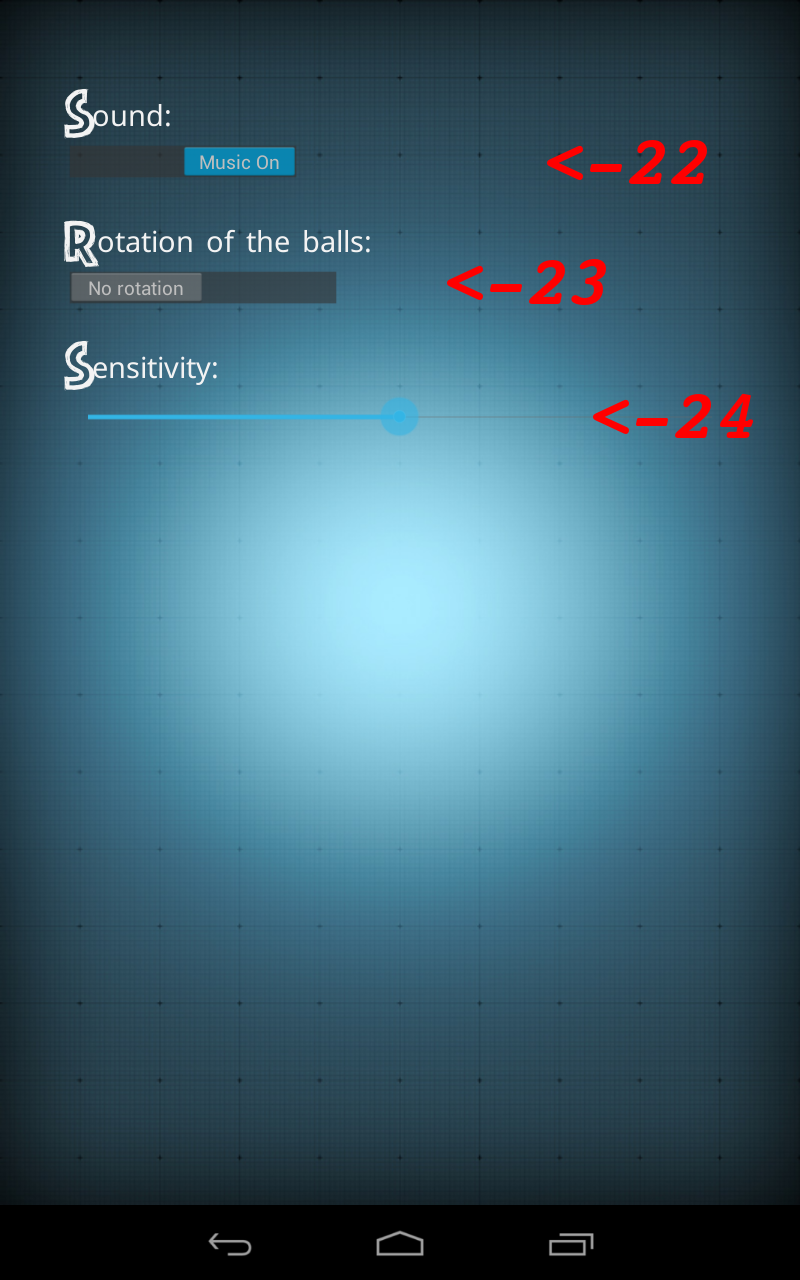
\includegraphics[scale=0.15]{9_GlobalSettings.png}}
\end{figure}


\begin{multicols}{3}
\begin{enumerate}
\item Play button
\item Settings button
\item Highscore button
\item World selector
\item Level
\item Score
\item Remaining lives
\item Remaining time
\item Gameboard
\item Next level button
\item Menu button
\item Retry button
\item Restart button
\item User settings button
\item Global settings button
\item About button
\item User selector
\item New user creator
\item Bouboule selector
\item Tutorial switch
\item Reset game button
\item Sound switch
\item Rotation switch
\item Sensitivity selector
\end{enumerate}
\end{multicols}


\section*{How to?}

	\subsection*{How to create a new user profile?}
First, on the menu, select the settings menu (2), then the user section (14). Write your player name in the new user creator (18), then validate it by pressing the enter button. Your new profile is now created! You can remark it on the user selector (17) where the current player is always on top.

!! Warning !! : you can't choose already taken names, names containing specials characters or any special combination of characters that are invalid files names. But don't worry, a notification will appear if you input a bad user name.

Now you can go back to the main menu to play or stay in this menu to personalise your profile.

	\subsection*{How to change current user profile?}
	
In the user settings menu (14), click on the user selector (17). A list of the different potential users is displayed. Select your profile by clicking on it. It will appear on the top of the user selector (17).

Now you have selected your profile, you can go back to the main menu to play or stay in this menu to personalise your profile.

	\subsection*{How to personalise my profile?}

First, select the user settings menu (14). Check the user selector (17), to be sure to customize the right profile.\\
You are able to do several changes.

		\subsubsection*{Change the character skin}

With the Bouboule selector (19) you are able to change the Bouboule skin you are playing with. You can only embody Bouboule you have already defeated so if you can't switch, go play and win games to win new skins.

		\subsubsection*{Tutorial}

A little tutorial is display on the screen the first time you play the first level. If you want to see it again just change the tutorial switch (20).

!! Warning !! : If reset the tutorial, your current save game will be lost.

		\subsubsection*{Reset}
		
If you want to reset your last saved game just press the reset button (21) and it will be done.

	\subsection*{How to play?}

In the main menu, click on play (1). You have now access to the world selector (4). Just swipe between worlds and select one to begin the game. If you quitted the game during a match, the last saved game will be automatically restarted. \\


When you are playing just tilt the device to control the Bouboule. And don't forget, the aim is to push the enemy outside the arena, but pay attention, don't throw yourself out. \\

During the game, you can see witch level you are playing (5), what's your current score (6), how many lives remains (7) and how much time is left to end the level (8).\\

When you win a battle, you arrive at the winning screen where you can see the score (6) and your remaining lives (7). You can now go to the next level (10) or go back to the main menu (11) to quit the game. \\

If you lose your battle, you arrive on the losing screen. You can see your score (6) and your remaining lives (7). You can either retry the battle (12) or go the main menu (11). \\

When you lose and don't have remaining lives you go to the game over sceen. Your score is display (6). If your score is high enough it will be added to the high-score (you can view it went you are on the main menu by clicking on the high-score button (3)). At this point you can restart a game (13) (the world selector (4) will be displayed) or selected the main menu (11).

	\subsection*{How to pause the game?}

	When you are in game, just press back and the game will be paused. You can then choose to resume the game, go the the main menu or quit the application. Your current game progression will be saved and resume the next time you play (unless you reset the game).
	
	\subsection*{Some other settings}

	If you go in the global settings menu (from the main menu, go to settings (2) and then to global settings (15)), you can also choose if you want music/effects (22) or if you want that the Bouboule rotate (23). You can also move the sensibility of the device (24).







\end{document}
